\subsubsection{\ac{ATIS} and GeoQuery}
\label{sec:atis}

ATIS \cite{dahl-etal-1994-expanding} and GeoQuery \cite{10.1007/3-540-44795-4_40} are two datasets that are frequently utilized for semantic parsing, a technique for converting natural language inquiries into a structured meaning representation. The ATIS dataset consists of audio recordings and hand transcripts of individuals using automated travel inquiry systems to search for information regarding flights. It is structured using a relational schema to organize data from the official airline guide, with 25 tables containing information concerning fares, airlines, flights, cities, airports, and ground services.
All questions concerning this dataset can be answered using a single relational query. This makes it an ideal choice for training deep learning models, as it is designed for a specific domain and the queries are relatively straightforward.

Furthermore, the questions in the ATIS dataset \cite{dahl-etal-1994-expanding} are mainly limited to select and project queries. On the other hand, GeoQuery \cite{10.1007/3-540-44795-4_40} is made up of seven tables from the US geography database and 880 natural languages to SQL pairings. It includes geographic and topographical characteristics such as capitals, populations, and landforms. While both datasets are regularly employed to train deep learning models, GeoQuery \cite{10.1007/3-540-44795-4_40} is more comprehensive and provides a wider range of queries than ATIS. This includes JOIN and nested queries, as well as grouping and order queries, which are absent in the ATIS dataset\cite{dahl-etal-1994-expanding}. As a result, GeoQuery is better equipped to answer more complex queries, making it a better choice for training AI models.

% A relational schema is used to organize data from the official airline guide in the ATIS corpus. There are 25 tables containing information about fares, airlines, flights, cities, airports, and ground services. All questions related to this dataset can be answered using a single relational query. The relational database uses shorter tables for this dataset to answer queries intuitively.

% Here is an example query from the ATIS dataset: Input is in natural language, and the output is in \lambda calculus.

% \begin{figure}[H]
%     \centering
%     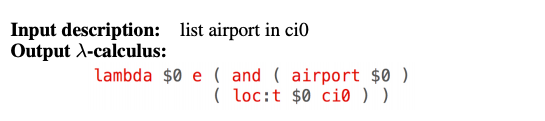
\includegraphics[width=0.8\textwidth]{pics/db/ATIS.png}
%     \caption{Example from ATIS dataset for semantic parsing}
%     \label{fig:ATIS}
% \end{figure}

% \subsubsection{GeoQuery Dataset}

% United States geography is represented in the Geoquery dataset. About 800 facts are expressed in Prolog. State, city, river, and mountain information can be found in the database. Geographic and topographical attributes such as capitals and populations make up the majority of the attributes.

% \begin{table}[H]
%     \centering
%     \caption{Example of a complex ATIS SQL query}
%     \label{tab:ATISsqlquery}
%     \begin{tabular}{|l|p{10cm}|}
%         \hline
%         Text & I would like a flight between BOSTON and ATLANTA on any day at one in the afternoon.                                                                                                                                                                                                                                                                                                                                                                                                                                    \\ \hline
%         SQL  & \small\texttt{SELECT DISTINCT flight.FLIGHT\_ID FROM AIRPORT\_SERVICE AS airport\_service , AIRPORT\_SERVICE AS airport\_service2 , CITY AS city2 , CITY AS city , FLIGHT AS flight WHERE ( city.CITY\_CODE = airport\_service2.CITY\_CODE AND city.CITY\_NAME = "ATLANTA" AND flight.DEPARTURE\_TIME = 1300 AND flight.TO\_AIRPORT = airport\_service2.AIRPORT\_CODE ) AND city2.CITY\_CODE = airport\_service.CITY\_CODE AND city2.CITY\_NAME = "BOSTON" AND flight.FROM\_AIRPORT = airport\_service.AIRPORT\_CODE ;} \\ \hline
%     \end{tabular}
% \end{table}

\begin{figure}[H]
    \label{tab:ATIS}
    \begin{AIbox}{Example of a complex ATIS SQL query}
        \vspace{-5px}
        \parbox{1\textwidth}{\scriptsize
        \begin{alltt} \larger
            {\bf Utterance:} \\ 
            I would like a flight between BOSTON and ATLANTA on any day at one in the afternoon. 
            \\
            {\bf Query:} \\
            SELECT DISTINCT flight.FLIGHT\_ID FROM AIRPORT\_SERVICE AS airport\_service , AIRPORT\_SERVICE AS airport\_service2 , CITY AS city2 , CITY AS city , FLIGHT AS flight WHERE ( city.CITY\_CODE = airport\_service2.CITY\_CODE AND city.CITY\_NAME = "ATLANTA" AND flight.DEPARTURE\_TIME = 1300 AND flight.TO\_AIRPORT = airport\_service2.AIRPORT\_CODE ) AND city2.CITY\_CODE = airport\_service.CITY\_CODE AND city2.CITY\_NAME = "BOSTON" AND flight.FROM\_AIRPORT = airport\_service.AIRPORT\_CODE ;
        \end{alltt}
        }
        \vspace{-5px}
    \end{AIbox}
    \captionsetup{font={scriptsize,color=white}, skip=-20pt}
    \caption{Example of a complex ATIS SQL query}
\end{figure}